Da bei vielen elektrischen und physikalischen Systemen das Rauschen zunimmt, wenn
die Frequenz $\omega$ gegen 0 strebt \cite{enet}, wird ein Lock-in-Verstärker
verwendet, um das Signal zu verstärken. Mit dieser Technik können dann auch
Signale mit niedrigen Frequenzen detektiert werden. Um dies zu erreichen, wird die
zu messende Frequenz mit einer Referenzfrequenz $\omega_0$ moduliert. \\
\begin{figure}[h]
  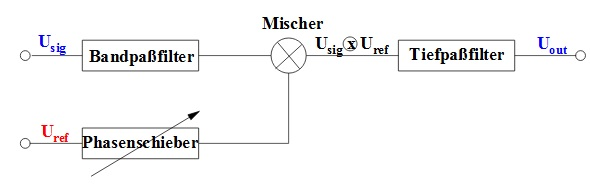
\includegraphics{Bilder/Schema.jpeg}
  \caption{schematischer Aufbau}
  \label{fig:schema}
\end{figure} \\
Abbildung \ref{fig:schema} zeigt den schematischen Aufbau eines Lock-In-Verstärkers.
Das verrauschte Nutzssignal $U_{sig}$ wird zuerst durch einen Bandpass-Filter
von Rauschanteilen mit hoher beziehungsweise niedriger Frequenz befreit, bevor
es in einem Mischer mit dem Referenzsignal $U_{ref}$ mit der Frequenz $\omega_0$
multipliziert. Die Phasenlage $\Phi$ von $U_{ref}$ lässt sich mit dem
Phasenschieber variieren und kann so mit der Signalspannung synchronisiert werden,
sodass $\Delta\Phi =0$.
Der nachgeschaltete Tiefpass-Filter integriert das Mischsignal $(U_{sig}\times U_{ref})$
mit einer Zeitkonstanten $\tau = RC \gg 1/\omega_0$.
Rauschbeiträge, die nicht mit der Modulationsspannung synchronisiert sind, werden
hierbei herausgemittelt. Somit erhält man eine zur Eingangsspannung proportionale
Ausgangsspannung $U_{out} \propto U_0 \cos{\Phi}$.
Je größer die Zeitkonstante $\Tau =RC$ gewählt wird, desto kleiner kann die
Bandbreite $\Delta v=1/(\pi RC)$.
Der Gütefaktor der bei Lock-In-Verstärkern erreicht wird liegt bei Q=100000
\cite{303}. \\
\begin{figure}[p]
  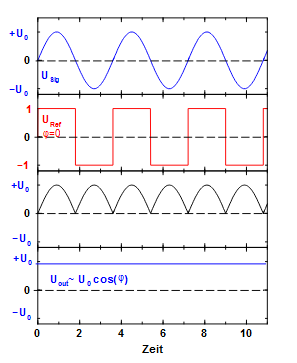
\includegraphics{Bilder/Spannung.jpeg}
  \caption{Spannungsverläufe}
  \label{fig:spannung}
\end{figure}
